%%%%%%%%%%%%%%%%%%%%%%%%%%%%%%%%%%%%%%%%%%%%%%%%%%%%%%%%%%%%%%%%%%%%%%%%%%%%
%
%  Template code for the Undergraduate Research Scholars thesis program starting, updated by Undergraduate Research Scholars program staff. Version 6.0. Last Updated: Fall 2024
%  Modified by Tawfik Hussein from the template code for TAMU Theses and Dissertations starting Spring 2018, authored by Sean Zachary Roberson. Version 3.17.09.
%
%
%%%%%%%%%%%%%%%%%%%%%%%%%%%%%%%%%%%%%%%%%%%%%%%%%%%%%%%%%%%%%%%%%%%%%%%%%%%%%%%

%%%%%%%%%%%%%%%%%%%%%%%%%%%%%%%%%%%%%%%%%%%%%%%%%%%%%%%%%%%%%%%%%%%%%%%%%%%
%%                           APPENDIX 
%%%%%%%%%%%%%%%%%%%%%%%%%%%%%%%%%%%%%%%%%%%%%%%%%%%%%%%%%%%%%%%%%%%%%%%%%%%

% The Appendix section is optional, must be placed directly after the references section, can be a collection of large data sets, images, and/or tables tghat would interrupt a significant portion of your writing. It can be a single Appendix (label as Appendix: Title) or it can include multiple Appendices (label as Appendix A: Title, Appendix B: Title, etc). Label figures, tables, and equations consecutively starting with A.1, A.2, etc. For additional Appendices (B, C, etc.), label figures, tables, and equations as B.1, B.2, etc. It can also be as many pages as needed.

%_________(0)____________

% Do not modify this section. This ensures proper formatting of the appendix tables, equations, and figures.

\phantomsection

\chapter*{\large\bf APPENDIX: TITLE}
\addcontentsline{toc}{chapter}{APPENDIX: TITLE} 

% These two lines reset the counter for figures and adds an "A" before each figure number (i.e, Figure A.1)

\renewcommand{\thefigure}{A.\arabic{figure}}
\setcounter{figure}{0}

% These two lines reset the counter for tables and adds an "A" before each figure number (i.e, tables A.1)
\renewcommand{\thetable}{A.\arabic{table}}
\setcounter{table}{0}

\renewcommand{\theequation}{A.\arabic{equation}}
\setcounter{equation}{0}

%___________(1)____________
% Modifications needed! 

% [INSTRUCTIONS FOR REQUIRED ACKNOWLEDGEMENTS PAGE.]

%The Appendix section: 
%\begin{itemize}
%  \item Is optional
%  \item Must be placed directly after the References section
%  \item Can be a collection of large data sets, images, and/or tables that would interrupt a significant portion of your writing
%  \item Can be a single Appendix (label as Appendix: Title)
%  \item Can include multiple Appendices (label as Appendix A: Title, Appendix B: Title, etc.)
%  \item Label figures, tables, and equations consecutively starting with A.1, A.2, etc. For additional Appendices (B, C, etc.), label figures, tables, and equations as B.1, B.2, etc.
%  \item Can be as many pages as needed
%\end{itemize}

%____________(2)_________________
% MODIFY THE SAMPLE APPENDIX PAGE. INCLUDES EXAMPLE FIGURES WITH PROPER CAPTION LABELLING AND NUMBERING. 
[Type content here.]

\begin{table}[htp]
    \centering
    \caption{Call this table A.1.}
    \label{tab1}
  	\begin{tabular}{|l|l|l|l|}  % Each "l" corresponds to a column in the table. Hence, the total number of "l"
	                            % corresponds to the number of columns your table will have.
		\hline
		\bf{Heading 1} & \bf{Heading 2} & \bf{Heading 3} & \bf{Heading 4} \\ \hline
		Content example. & Content example. & Content example. & Content example. \\ \hline
		Content example. & Content example. & Content example. & Content example. \\ \hline
    \end{tabular}
\end{table}

\begin{figure}[H]
\centering    % This centers it
	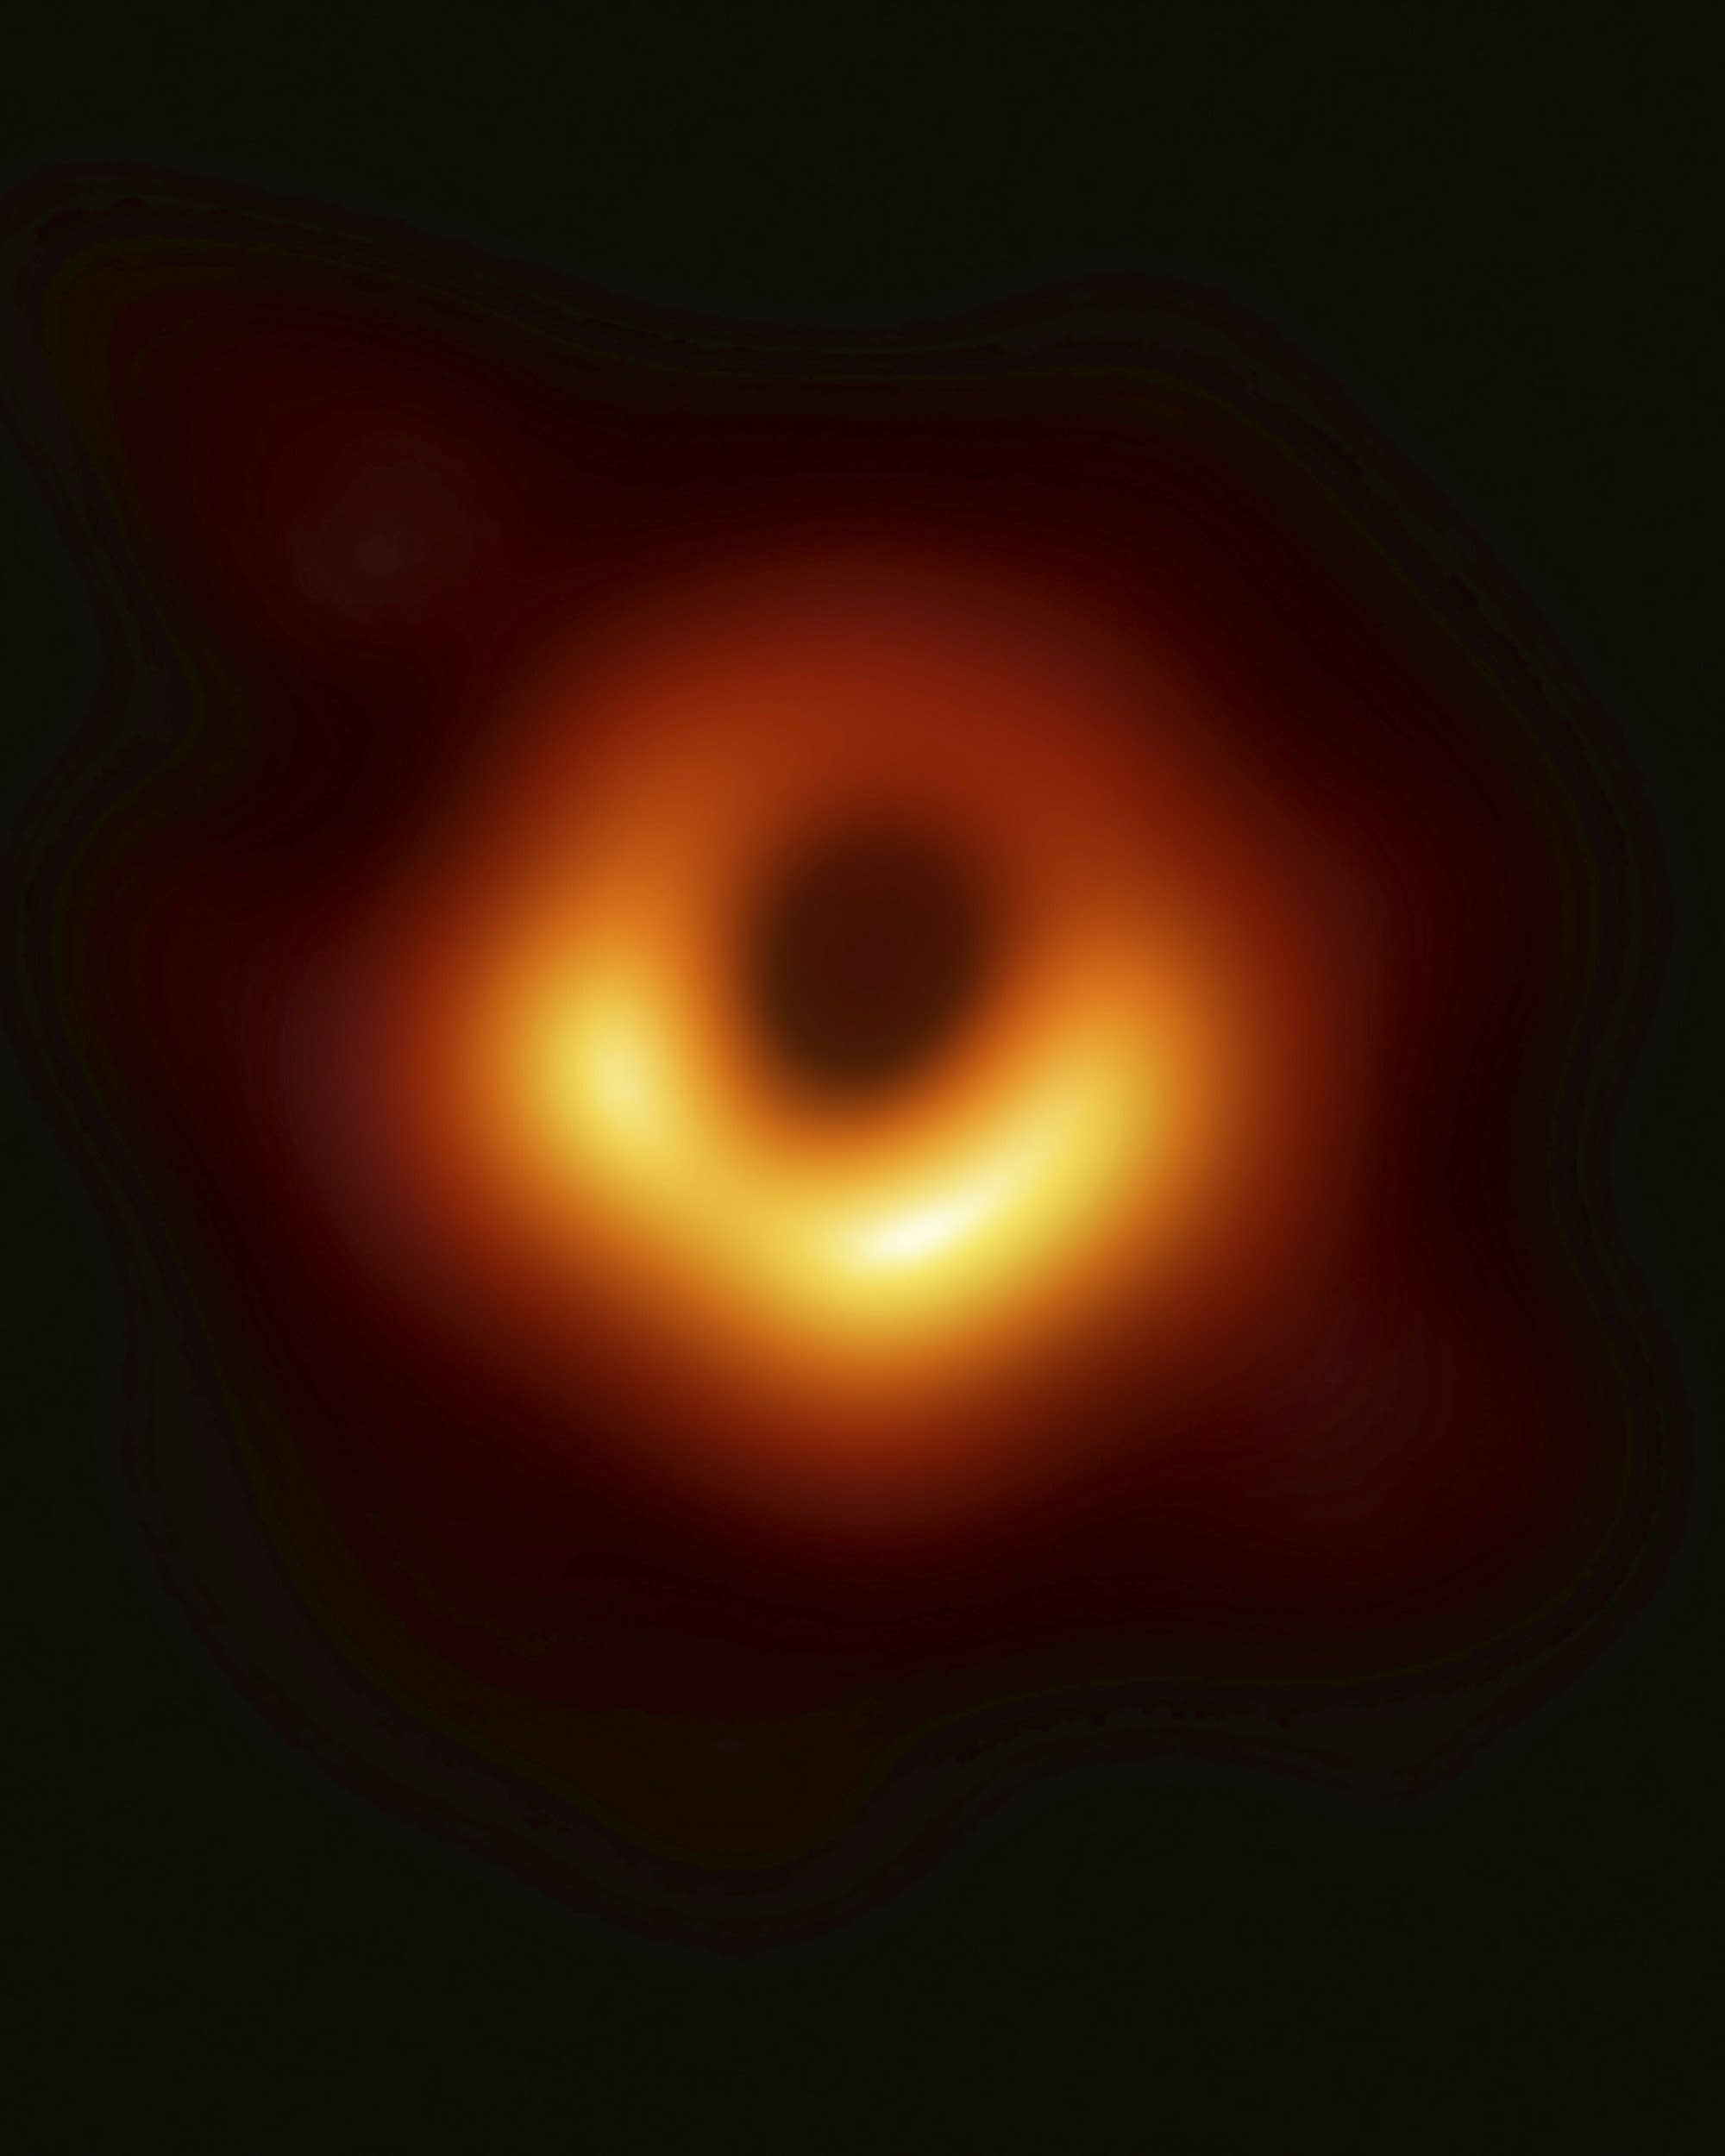
\includegraphics[scale=0.10]{figures/blackhole.jpg}
	\captionsetup{justification=centering}
	\captionsetup{format=hang}
        \singlespace
	\caption{The first recorded image of a black hole}    % This is the caption of the figure
%\label{figa2}
\end{figure}

\begin{equation} \label{Equ.A.1}
R_{\mu \nu} - {\frac{1}{2}}g_{\mu \nu}\,R + g_{\mu \nu} \Lambda = 
 {\frac{8 \pi G}{c^4}} T_{\mu \nu}
\end{equation}